\section{马尔科夫链}

\begin{frame}
  \frametitle{马尔科夫链概述}
  \begin{itemize}
    \item 马尔科夫链假设某一时刻状态转移的概率只依赖于它的前一个状态。
    \item 这样假设可以大大简化模型的复杂度,因此马尔科夫链在很多时间序列模型中得到广泛的应用,比如循环神经网络RNN,隐式马尔科夫模型HMM等,MCMC也需要它。
    \item 用精确的数学定义来描述,则假设我们的序列状态是$..., X_{t-2}, X_{t-1}, X_t, X_{t+1}, X_{t+2},...$,
    那么我们的在时刻$t+1$的状态的条件概率仅仅依赖于时刻$t$,即:
    $$P(X_{t+1}|...,X_{t-2},X_{t-1},X_t) = P(X_{t+1}|X_t)$$
    \item 既然某一时刻状态转移的概率只依赖于它的前一个状态,那么我们只要能求出系统中任意两个状态之间的转换概率,这个马尔科夫链的模型就定了。
    我们来看看下图这个马尔科夫链模型的具体的例子(来源于维基百科)。
  \end{itemize}
\end{frame}

\begin{frame}
  \frametitle{马尔科夫链概述}
  \begin{figure}
    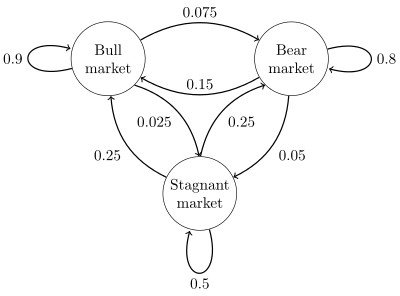
\includegraphics[trim=0 0 0 0,clip,height=5cm]{mcmc/niuxiongshi.png}
    \caption{马尔科夫链是表示股市模型}
  \end{figure}
\end{frame}

\begin{frame}
  \frametitle{马尔科夫链概述}
  \begin{itemize}
    \item 这个马尔科夫链是表示股市模型的,共有三种状态:牛市(Bull market), 熊市(Bear market)和横盘(Stagnant market)。
    \item 每一个状态都以一定的概率转化到下一个状态。比如,牛市以0.025的概率转化到横盘的状态。
    这个状态概率转化图可以用矩阵的形式表示。如果我们定义矩阵阵$P$某一位置$P(i,j)$的值为$P(j|i)$,即从状态$i$转化到状态$j$的概率,
    并定义牛市为状态0, 熊市为状态1, 横盘为状态2。这样我们得到了马尔科夫链模型的状态转移矩阵为:
    \begin{equation*}
      P = 
      \begin{pmatrix}
        0.9 & 0.075 & 0.025 \\
        0.15 & 0.8 & 0.05  \\
        0.25 & 0.25 & 0.5 \\
      \end{pmatrix}
    \end{equation*}
  \end{itemize}
\end{frame}

\begin{frame}
  \frametitle{马尔科夫链模型状态转移矩阵的性质}
  \begin{itemize}
    \item 马尔科夫链模型的状态转移矩阵收敛到的稳定概率分布与初始状态概率分布无关。
    这是一个非常好的性质,也就是说,如果我们得到了这个稳定概率分布对应的马尔科夫链模型的状态转移矩阵,
    则我们可以用任意的概率分布样本开始,带入马尔科夫链模型的状态转移矩阵,这样经过一些序列的转换,最终就可以得到符合对应稳定概率分布的样本。
    \item 如果一个非周期的马尔科夫链有状态转移矩阵$P$, 并且它的任何两个状态是连通的,那么$\lim_{n \to \infty} P_{ij}^n$与$i$无关,我们有:
  \end{itemize}

\end{frame}

\begin{frame}
  \frametitle{}
  \begin{enumerate}
    \item $$\lim_{n \to \infty} P_{ij}^n = \pi(j)$$
    \item $$\lim_{n \to \infty} P_{ij}^n = 
    \begin{pmatrix}
      \pi(1) &\pi(2)&...&\pi(3)&...\\
      \pi(1) &\pi(2)&...&\pi(3)&...\\
      ... &...&...&...&...\\
      \pi(1) &\pi(2)&...&\pi(3)&...\\
      ... &...&...&...&...\\
    \end{pmatrix}
    $$
    \item 
  \end{enumerate}
  
\end{frame}

\begin{frame}
  \frametitle{}
  \begin{enumerate}
    \item $$\pi(j) = \sum_{i=0}^\infty \pi(i)P_{ij}$$
    \item $\pi$ 是方程$\pi P = \pi$的唯一非负解,其中:$$\pi = [\pi(1), \pi(2),...,\pi(j), ...] \sum_{i=0}^\infty \pi(i) = 1$$
  \end{enumerate}
  
\end{frame}

\begin{frame}
  \frametitle{基于马尔科夫链采样}
  
\end{frame}